%! Author = omar
%! Date = 2/22/24

% Preamble
\documentclass[11pt]{article}

\title{Astrodynamics Study}
\author{Omar Crosby}

% Packages
\usepackage{amsmath}
\usepackage{xcolor} % Include the xcolor package for coloring text
\usepackage{amsthm} % Include the amsthm package for theorem-like environments
\usepackage{graphicx} % Include the graphicx package for including images
\usepackage{siunitx}
\usepackage{enumitem}

% Document
\begin{document}

    \maketitle

    \section{Kepler's Laws}

    \begin{figure}[h]
        \centering
        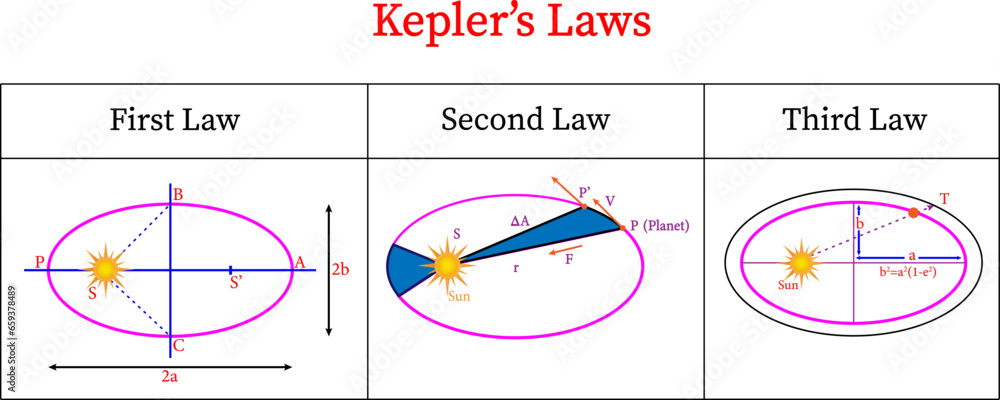
\includegraphics[width=\textwidth]{images/keplers_laws.jpeg}
        \caption{Kepler's Laws}
        \label{fig:keplers_laws}
    \end{figure}

    Kepler published his first two laws of planetary motion in 1609 and the third law in 1619.  He spent from 1601
    until 1606 trying to fit various geometrical curves to the measurements from the Danish noble Tycho Brahe. The
    three laws are as follows:

    \subsection{First Law}
    The orbit of each planet is an ellipse, with the Sun at a focus.

    \subsection{Second Law}
    The line joining the planet to the sun sweeps out equal areas in equal times.

    \subsection{Third Law}
    The square of the period of a planet is proportional to the cube of its mean distance from the Sun.  The semi-major axis of the ellipse is also called the mean distance from the Sun.

    \section{Newton's Laws of Motion}

    \subsection{First Law}
    Every body continues in its state of rest or of uniform motion in a straight line unless it is complelled to change that state by forces impressed upon it.

    \subsection{Second Law}
    The time-rate of change of momentum is proportional to the force impressed and is in the same direction as that force.

    \begin{equation}
        \mathbf{F} \propto \dot{\rho}
        \label{eq:newtons_second_law_proportion}
    \end{equation}

    \subsection{Third Law}
    To every action there is always opposed an equal reaction.

    The second law can be expressed mathematically as follows:

    \begin{equation}
        \sum \mathbf{F} = m \ddot{\mathbf{r}}
        \label{eq:newtons_second_law}
    \end{equation}

    where $\sum \mathbf{F}$ is the vector sum of all the forces acting on the mass and is the vector acceleration of the
    mass measured relative to an inertial reference frame. Note that equation\ \ref{eq:newtons_second_law}, applies only for a system of
    constant mass.

    \section{Newton's Law of Universal Gravitation}

    In Book 1 of \textit{The Mathematical Principles of Natural Philosophy}, Sir Isaac Newton introduced his
    three laws of motion. Also in /textit{The Principia}, Newton formulated the law of gravity by stating that
    any two bodies attract one another with a force proportional to the product of their masses and inversely
    proportional to the square of the distance between them.

    \begin{equation}
        \mathbf{F}_{g} \propto m M
        \label{eq:gravitational_force_proportion}
    \end{equation}

    \begin{equation}
        \mathbf{F}_{g} \propto \frac{1}{r^2}
        \label{eq:gravitational_force_distance}
    \end{equation}

    \begin{equation}
        \mathbf{F}_{g} = -G \frac{m M}{r^2} \frac{\mathbf{r}}{r}
        \label{eq:gravitational_force}
    \end{equation}

    where $\mathbf{F}_{g}$ is the force on mass \textbf{m} due to mass \textbf{M} and $\mathbf{r}$ is the vector from
    M to m.  The universal gravitational constant, \textbf{G}, has the approximate value of

    \begin{equation}
        G = 6.673 \times 10^{-20} \, \frac{\text{km}^3}{\text{kg} \times \text{s}^{2}}
    \end{equation}

    \section{The n-Body Problem}

    Within the n-body problem we consider the motion of a body (an earth satellite, a lunar or interplanetary probe, or
    a planet).  At any given time the body is being acted upon by several masses and may be expriencing other forces
    such as:

    \begin{enumerate}[label=\alph*)]
        \item Drag
        \item Thrust
        \item Solar Radiation Pressure
        \item Perturbations due to non-spherical shapes
    \end{enumerate}

    \subsection{A System of Bodies}

    We assume a "system" of n-bodies (${m}_{1}$, ${m}_{2}$, ${m}_{3}$, ..., ${m}_{n}$) one of which is the body whose
    motion we wish to study, call it the ${i}^{th}$ body ${m}_{i}$.  The vector sum of all gravitational forces and
    other external forces acting on ${m}_{i}$ will be used to determine the equation of motion.  To determine the
    gravitational forces we shall apply Newton's law of universal gravitation.  In addition, the ${i}^{th}$ body may
    be a rocket expelling mass (i.e. propellants) to produce thrust; the motion may be in an atmosphere where drag
    effects are present; solar radiation may impart some pressure on the body; etc.  All of these effects must be
    considered in the general equation of motion. An important force, not yet determined, is due to the nonspherical
    shape of the planets. The magintude of this force for near-Earth satellites are on the order of ${10}^{-3} g$.
    Although small, this force is responsible for several important effects not predictable from the studies of Kepler
    and Newton.

    Some of these wierd effects.

    \begin{enumerate}[label=\alph*)]
        \item line-of-nodes
        \item rotation of the line-of-apsides
    \end{enumerate}

    All of these effects must be considered in the general equation of motion.

    The first step in our analysis will be to choose a "suitable" coordinate system in which to express the motion.

    If the positions of the n masses are known: $\mathbf{r}_{1}$, $\mathbf{r}_{2}$, $\mathbf{r}_{3}$, \ldots, $\mathbf{r}_{n}$,
    then by applying Newton's law of universal gravitation, the force $\mathbf{{F}_{g_n}}$ exerted on ${m}_{i}$ by
    ${m}_{n}$ is given by:

    \begin{equation}
        \mathbf{{F}_{g_n}} = -\frac{{G} {m}_{i} {m}_{n}}{r_{ni}^{3}} \mathbf{r}_{ni}
        \label{eq:force_on_m_i}
    \end{equation}

    Where $\mathbf{{F}_{g_n}}$ is the force excerted on ${m}_{i}$ by ${m}_{n}$, and

    \begin{equation}
        \mathbf{r}_{ni} = \mathbf{r}_{i} - \mathbf{r}_{n}
        \label{eq:vector_r_ni}
    \end{equation}

    The vector sum $\mathbf{F}_{g}$, of all such gravitational forces acting on the ${i}^{th}$ body is given by:

    \begin{equation}
        \mathbf{F}_{g} = -G m_{i}\sum_{\substack{j=1 \\ j \neq i}}^{n} \frac{m_{j}}{r_{ji}^{3}} \mathbf{r}_{ji}
        \label{eq:vector_sum_gravitational_forces}
    \end{equation}


    \begin{equation}
        \mathbf{F}_{TOTAL} = \mathbf{F}_{g} + \mathbf{F}_{OTHER}
        \label{eq:total_force}
    \end{equation}

    \vspace{10mm} % Adds a space of 10mm before the next paragraph

    The other external force $\mathbf{F}_{OTHER}$ is composed of drag, thrust, solar radiation pressure,
    perturbations due to non-spherical shapes, etc.

    \vspace{10mm} % Adds a space of 10mm before the next paragraph

    Applying Newton's second law of motion

    \begin{equation}
        \frac{d}{dt} ({m}_{i} \mathbf{v}_{i}) = \mathbf{F}_{TOTAL}
        \label{eq:total_force_newtons_second_law}
    \end{equation}

    \vspace{10mm} % Adds a space of 10mm before the next paragraph

    where $\mathbf{v}_{i}$ is the velocity of the ${i}^{th}$ body.

    \vspace{10mm} % Adds a space of 10mm before the next paragraph

    The time derivative may be expanded to

    \begin{equation}
        {m}_{i} \frac{d\mathbf{v}_{i}}{dt} + \mathbf{v}_{i} \frac{d{m}_{i}}{dt} = \mathbf{F}_{TOTAL}
        \label{eq:time_derivative_expansion}
    \end{equation}

    \vspace{10mm} % Adds a space of 10mm before the next paragraph

    Dividing through by the mass ${m}_{i}$ gives the most general equation for the motion for the ${i}^{th}$ body:

    \begin{equation}
        \ddot{\mathbf{r}_{i}} + \frac{\mathbf{r}_{i}}{dt} = \frac{\mathbf{F}_{TOTAL}}{m_{i}}
        \label{eq:general_equation_motion}
    \end{equation}

    \vspace{10mm} % Adds a space of 10mm before the next paragraph

    or

    \vspace{10mm} % Adds a space of 10mm before the next paragraph

    \begin{equation}
        \ddot{\mathbf{r}_{i}} = \frac{\mathbf{F}_{TOTAL}}{m_{i}} - \dot{\mathbf{r}_{i}} \frac{\dot{m}_{i}}{m_{i}}
        \label{eq:general_equation_motion_simplified}
    \end{equation}

    where

    \begin{enumerate}[label=\alph*)]
        \item $\ddot{\mathbf{r}_{i}}$ is the acceleration of the ${i}^{th}$ body,
        \item ${m}_{i}$ is the mass of the ${i}^{th}$ body, and
        \item $\mathbf{F}_{TOTAL}$ is the vector sum of all gravitational forces given by
    \end{enumerate}

    \begin{equation}
        \mathbf{F}_{g} = -G m_{i}\sum_{\substack{j=1 \\ j \neq i}}^{n} \frac{m_{j}}{r_{ji}^{3}} \mathbf{r}_{ji}
        \label{eq:vector_sum_gravitational_forces_2}
    \end{equation}

    \vspace{10mm} % Adds a space of 10mm before the next paragraph

    and all other external forces

    \begin{equation}
        \mathbf{F}_{OTHER} = \mathbf{F}_{DRAG} + \mathbf{F}_{THRUST} + \mathbf{F}_{SOLAR} + \mathbf{F}_{PERTURB}
        \label{eq:other_external_forces}
    \end{equation}

    \vspace{10mm} % Adds a space of 10mm before the next paragraph

    Note that $\dot{{m}_{i}}$ is the time rate of change of the mass of the ${i}^{th}$ body (due to expelling mass
    or relativistic effects).

    \vspace{10mm} % Adds a space of 10mm before the next paragraph

    As a rocket burns fuel it's mass decreases causing the mass to decrease over time.

\end{document}

